
\documentclass[11pt,titlepage,a4paper]{report}

%INCLUSIONE PACCHETTI
%---------------------------------------------
\usepackage[italian]{babel}
\usepackage{fancyhdr}
\usepackage{graphicx}
\graphicspath{{./pics/}} % cartella di salvataggio immagini

% STILE DI PAGINA
%---------------------------------------------
\pagestyle{fancy}
\renewcommand{\sectionmark}[1]{\markright{\thesection.\ #1}}
\lhead{\nouppercase{\rightmark}}
\rhead{\nouppercase{\leftmark}}
\renewcommand{\chaptermark}[1]{%
\markboth{\thechapter.\ #1}{}}

%Ridefinisco lo stile plain della pagina
\fancypagestyle{plain}{%
	\lhead{
\includegraphics[height=50pt]{logo.eps}}
	\chead{}
	\rhead{HappyCode inc \\ happycodeinc@gmail.com}
	\lfoot{BR-jsys}
	\cfoot{\thepage}
	\renewcommand{\headrulewidth}{1pt}
	\renewcommand{\footrulewidth}{1pt}
}
% layout
\begin{document}
%definizione variabili 
\newcommand{\lv}{ 1.8 } % latest version
\newcommand{\dt}{ Piano Di Progetto }% Document title
\newcommand{\Glossario}{ Glossario.1.8.pdf }
%fine definizione variabili
%common variables
\newcommand{\br}{\underline{business rule}}
\newcommand{\brs}{\underline{business rules}}
\newcommand{\bo}{\underline{business object}}
\newcommand{\bos}{\underline{business objects}}
\newcommand{\rp}{\underline{repository}}
\newcommand{\brp}{BusinessRuleParser}
\newcommand{\brl}{BusinessRuleLexer}
\newcommand{\BR}{\underline{BusinessRule}}

%nomi dei componenti
\newcommand{\AT}{Alessia Trivellato}
\newcommand{\ET}{Elena Trivellato}
\newcommand{\FC}{Filippo Carraro}
\newcommand{\LA}{Luca Appon}
\newcommand{\MB}{Michele Bortolato}
\newcommand{\MT}{Marco Tessarotto}
\newcommand{\MM}{Mattia Meroi}%altre variabili
\hyphenation{
 a-na-lo-go
 as-so-cia-zio-ne
 %attività non si può inserire come tutte le parole accentate che vanno messe nel testo semplice scritte at\-ti\-vi\-tà o come variabile
 coe-ren-za
 com-po-nen-ti
 des-crit-te
 des-cri-zio-ni
 di-a-gram-ma
 di-a-gram-mi
 e-le-men-to
 e-se-gui-re
 e-si-sten-ti
 es-pli-ci-to
 glo-bal-men-te
 glos-sa-rio
 li-vel-lo
 ne-ces-sa-rio
 per-met-te-re
 re-po-si-to-ry
 re-vi-sio-na-men-to
 ri-chies-te
 se-gna-la-ta
 va-li-da-zio-ne
 va-ria-bi-li
 ve-ri-fi-ca-re
 vi-sua-liz-za-te
 e-ven-tua-li
 o-pe-ra-zio-ne
 ar-chi-via-zio-ne
 mo-di-fi-ca
}


%sillabazione
\begin{titlepage}
\begin{center}
\vspace*{0.5in}

\includegraphics{logo.eps}
\vspace*{0.2in}

{\Large \textbf{BR-jsys}}
{\Large \emph{business rules} per sistemi gestionali in architettura J2EE } 
\vspace{2in}

\Huge \textsc{ \dt }

\end{center}
\end{titlepage}
\vspace*{0.5in}%pagina del titolo


\begin{center}
\thispagestyle{plain}
\begin{table}[htbp]

\large{
\begin{tabular}{l}
\Large{\textbf{\textsf{Capitolato: ''BR-jsys``}}} \\
\begin{tabular}{|p{6cm}|p{6cm}|} \hline
\textbf{Data creazione:} & 2007/11/21 \\ \hline
\textbf{Versione:} & \lv \\ \hline
% ----------------------------------------------------------------------------autori
\textbf{Stato del documento:} & formale, esterno \\ \hline
\textbf{Revisione RR} &  \\ \hline
\textbf{Redazione:} & \ET \\ \hline
\textbf{Revisione:} & \MT \\ \hline
\textbf{Approvazione:} & \ET \\ \hline
\textbf{Revisione RPD} &    \\ \hline
\textbf{Redazione:} & \MM \\ \hline
\textbf{Revisione:} & \ET , \FC \\ \hline
\textbf{Approvazione:}  & \MM \\  \hline
\textbf{Revisione RQ} &    \\ \hline
\textbf{Redazione:} & \ET \\ \hline
\textbf{Revisione:} & \\ \hline
\textbf{Approvazione:}  & \\  \hline
\end{tabular} \\
\end{tabular}
}
\end{table}

\begin{table}[hbtp]
\large{
\begin{tabular}{l}
\Large{\textbf{\textsf{Lista di distribuzione}}} \\
\begin{tabular}{|p{6cm}|p{6cm}|} \hline
%  -------------------------------------------------------------lista di distribuzione
{HappyCode inc}& Gruppo di lavoro\\ \hline
{Tullio Vardanega, Renato Conte}& Committenti \\ \hline 
{Zucchetti S.r.l}& Azienda proponente\\ \hline
\end{tabular} \\
\end{tabular}
}
\end{table}
\begin{table}[hbtp]

\Large{\textbf{\textsf{Diario delle modifiche}}} \\
\begin{small}
\begin{tabular}[t]{|p{1,2cm}|p{1.9cm}|p{2.9cm}|p{5cm}|} \hline
Versione & Data & Autore & Descrizione \\ \hline
%-------------------------------------------------------------------------------diario modifiche
2.2 & 06/03/2008 & \ET & Aggiornamento diagrammi di Gantt\\ \hline
2.1 & 06/03/2008 & \MT & Aggiornamento grafici con dati effettivi della fase di sviluppo\\ \hline
2.0 & 06/03/2008 & \ET & Aggiornamento tabelle con dati effettivi della fase di sviluppo\\ \hline
1.9 & 05/03/2008 & \MM & Introduzione sottolineatura ai termini definiti nel glossario\\ \hline
1.8 & 04/03/2008 & \MT & Modifica al layout, introduzione totale pagine e autori nel diario delle modifiche.\\ \hline
1.7 & 14/02/2008 & \MM & Modifica ai grafici.\\ \hline
1.6 & 13/02/2008 & \MM & Aggiornamento tabelle con dati effettivi della fase di progettazione.\\ \hline
1.5 & 11/02/2008 & \MM & Modifica layout tabelle.\\ \hline 
1.4 & 05/02/2008 & \MT & Aggiunta del nome del file nel modello di documento.\\ \hline
1.3 & 25/01/2008 & \MM & Aggiornamento tabelle con dati effettivi della fase di analisi \\ \hline
1.2 & 23/01/2008 & \MM & Aggiunto carico totale delle risorse preventivo \\ \hline
1.1 & 22/01/2008 & \MT & Modifica al layout dei documenti.\\ \hline
1.0 & 21/12/2007 & \MT & Documento sottoposto a revisionamento automatico.\\ \hline
0.5 & 05/12/2007 & \ET & Aggiunto riferimento diagramma di Gantt \\ \hline
0.4 & 29/11/2007 & \ET & Stesura completa del documento. \\ \hline
0.3 & 25/11/2007 & \ET & Assegnazione dei ruoli ai componenti del gruppo. \\ \hline
0.2 & 23/11/2007 & \ET & Riviste al ribasso le ore di programmazione. \\ \hline
0.1 & 21/11/2007 & \ET & Stesura preliminare del documento. \\ \hline

\end{tabular} \\
\end{small}


\end{table}
\end{center}


\tableofcontents 


\chapter{Introduzione}
\section{Scopo del documento}
Questo documento rappresenta il piano di progetto preliminare/consuntivo del capitolato d'appalto per il sistema ``\underline{Business Rule} per sistemi gestionali in architettura \underline{J2EE} \underline{BR-jsys}''. Verr\`a qui riportata la suddivisione dei compiti e il costo complessivo del sistema, in base ai ruoli e alle ore impegnate.

\section{Glossario}
Il glossario viene fornito come file esterno chiamato \Glossario .

\section{Riferimenti}
\begin{itemize}
\item Capitolato d'appalto concorso per sistema ``\underline{BR-jsys}'';
\item Verbale dell'incontro con il proponente ``Incontro2007-11-22.pdf'';
\item Verbale dell'incontro con il proponente ``Incontro2008-02-05.pdf'';
\item ``Ingegneria del Software'' 8a edizione - Ian Sommerville.
\end{itemize}

\chapter{Ruoli}
\section{Definizione ruoli}
Nella tabella sottostante riportiamo l'impegno complessivo, in base ai ruoli di progetto, nelle quattro macrofasi previste dal ciclo di vita del nostro software. Quest'ultima
\`e stata aggiornata al 7 marzo, al termine della fase di sviluppo. Inseriamo quindi il valore effettivo di ore impiegate, riportando tra parentesi la differenza rispetto a quanto preventivato relativamente alle prime tre fasi. \\
Rispetto alle previsioni in fase di analisi sono aumentate considerevolmente 
le ore dei progettisti ed in fase di progettazione le ore 
dei programmatori, a scapito di quelle dei progettisti. Tutto ci\`o \`e avvenuto a seguito dell'utilizzo del generatore di parser che ha accelerato notevolmente i tempi, consentendoci di soffermarci di pi\`u sulla progettazione gi\`a in fase di analisi. Di conseguenza, in fase di progettazione abbiamo gi\`a a disposizione un piccolo prototipo software. 
\\In fase di sviluppo abbiamo quindi dovuto limitare il numero di ore per rientrare nei costi preventivati al cliente. Abbiamo deciso di limitare al minimo le ore di amministratore e responsabile (che sono tra i pi\`u costosi). Questo \`e stato possibile grazie al fatto che:
\begin{itemize}
\item il responsabile: ha delegato completamente all'amministratore l'aggiornamento del piano di progetto; 
\\l'approvazione del codice \`e stata snellita dai dettagliati rapporti sui test forniti dai verificatori; 
\\la pianificazione della qualit� in questa fase non ha subito particolari modifiche rispetto alle previsini fatte durante la fase precedente.
\item l'amministratore: non ha dovuto in questa fase mettere mano alle norme di progetto gi\`a sufficientemente esposte in modo chiaro e dettagliato nella fase precedente; 
\\ha ridotto al minimo la pianificazione di progetto che fatta eccezione per le modifiche ai ruoli di responsabile ed amministratore \`e rimasto pressoch\`e invariato rispetto all'ultima revisione;
\end{itemize}
Abbiamo altres\`i limitato le ore di verificatore in questa fase di sviluppo in quanto una parte dei test di verifica su interprete e GUI sono stati rimandati alla successiva fase di convalida quando le componenti saranno completate e pronte all'integrazione con il resto del prodotto.

\begin{table}[hbtp]
\large{
\begin{tabular}{l}
\Large{\textbf{\textsf{Tabella dei Ruoli}}} \\
\begin{tabular}{||p{3cm}||p{1.5cm}||p{1.5cm}||p{2cm}||p{1.5cm}||}
\hline 
\textbf{Ruoli} & \textbf{Analisi} & \textbf{Progett.} & \textbf{Sviluppo} & \textbf{Verifica}\\
\hline

{Responsabile}&10&10&7\footnotesize{(-3)} &9 \\ 
\hline 
{Amministratore} &10&10&8\footnotesize{(-2)}&10\\ 
\hline
{Analista}& 60 \footnotesize{(-2)}&20&5&0 \\
\hline
{Progettista}&29 \footnotesize{(+24)}&6 \footnotesize{(-15)}&25&0 \\
\hline
{Programmatore}&0&10 \footnotesize{(+5)}&59\footnotesize{(-1)}&55 \\
\hline
{Verificatore}& 30&30&85\footnotesize{(-5)}&95 \\
\hline
{Totale}& 137 \footnotesize{(+22)}&140 \footnotesize{(-10)}&189\footnotesize{(-11)}&169 \\
\hline
\end{tabular} \\

\end{tabular}
}

\end{table}

Il seguente grafico mostra in che misura incide ciascun ruolo per ogni macrofase. Abbiamo voluto mettere in evidenza le variazioni tra le nostre previsioni e il tempo effettivamente dedicato ad ogni ruolo, affiancando alle colonne con i colori pi\`u chiari (a destra, rappresentano i dati effettivi) le colonne che invece rappresentano i dati previsti (le abbiamo marcate con colori pi\`u scuri). Tale convenzione sar\`a usata anche nei grafici successivi. Per quanto riguarda la fase di verifica le due colonne (dati previsti/effettivi) coincidono, in quanto non siamo in possesso ancora di dati effettivi, trattandosi di fasi che affronteremo nell'immediato futuro.

\begin{center}
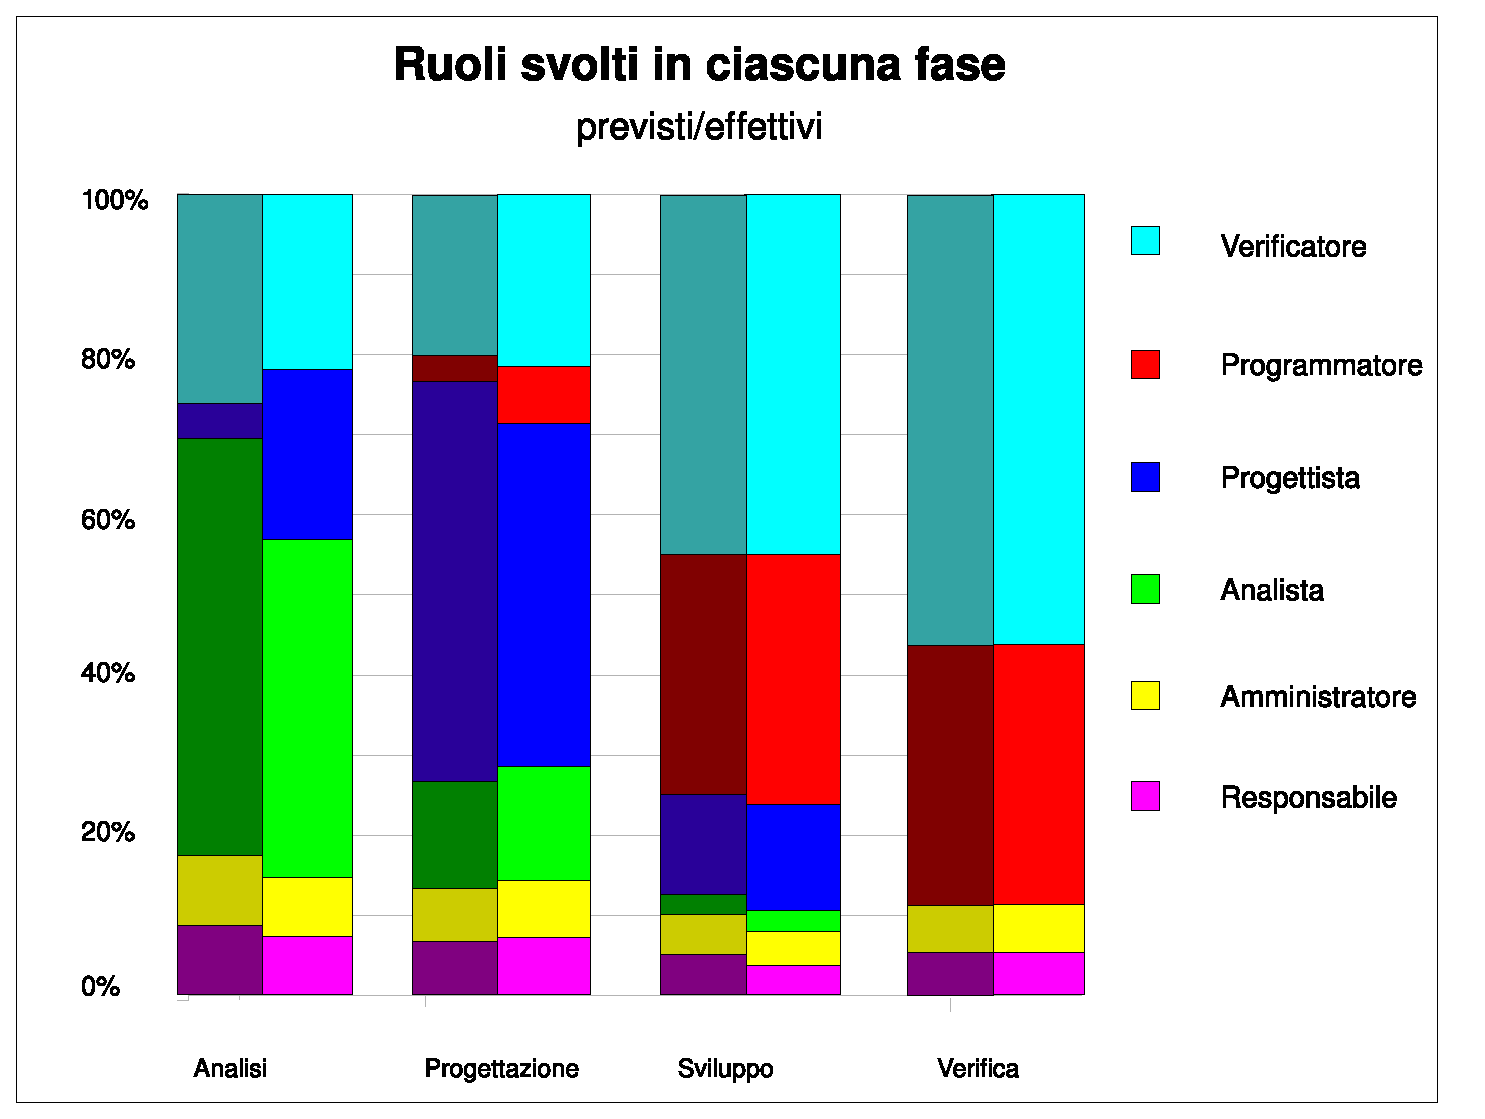
\includegraphics [width=1\textwidth] {progetto/confronto.eps}
\end{center}

\section{Incidenza percentuale}
Riportiamo in questa tabella il peso percentuale di ciascun ruolo nelle ore
complessive previste di realizzazione del prodotto. Le cifre tra parentesi indicano di quanto il dato effettivo riportato si discosta dalle previsioni iniziali.
\begin{table}[hbtp]
\large{
\begin{tabular}{l}
\Large{\textbf{\textsf{Tabella delle percentuali dei ruoli}}} \\
\begin{tabular}{||p{6cm}||p{4cm}||}
\hline

\textbf{Ruoli} & \textbf{Percentuali}\\
\hline
{Responsabile}&6\\ 
\hline 
{Amministratore} &6\\ 
\hline
{Analista} &13 \\
\hline
{Progettista} &18 \footnotesize{(+1)}\\
\hline
{Programmatore} &19\\
\hline
{Verificatore} &38 \footnotesize{(-1)} \\
\hline
{Totale} &100 \\
\hline

\end{tabular} \\
\end{tabular}
}
\end{table}

Evidenziamo la distribuzione delle ore, aggiornata al 7 marzo, tra i vari ruoli con un grafico. A differenza di prima abbiamo qui una visione globale riguardante tutto il ciclo di vita del software.
Anche in questo grafico a torta usiamo la convenzione che associa ai colori pi\`u scuri i dati previsti e a quelli pi\`u chiari i dati effettivi.


\begin{center}
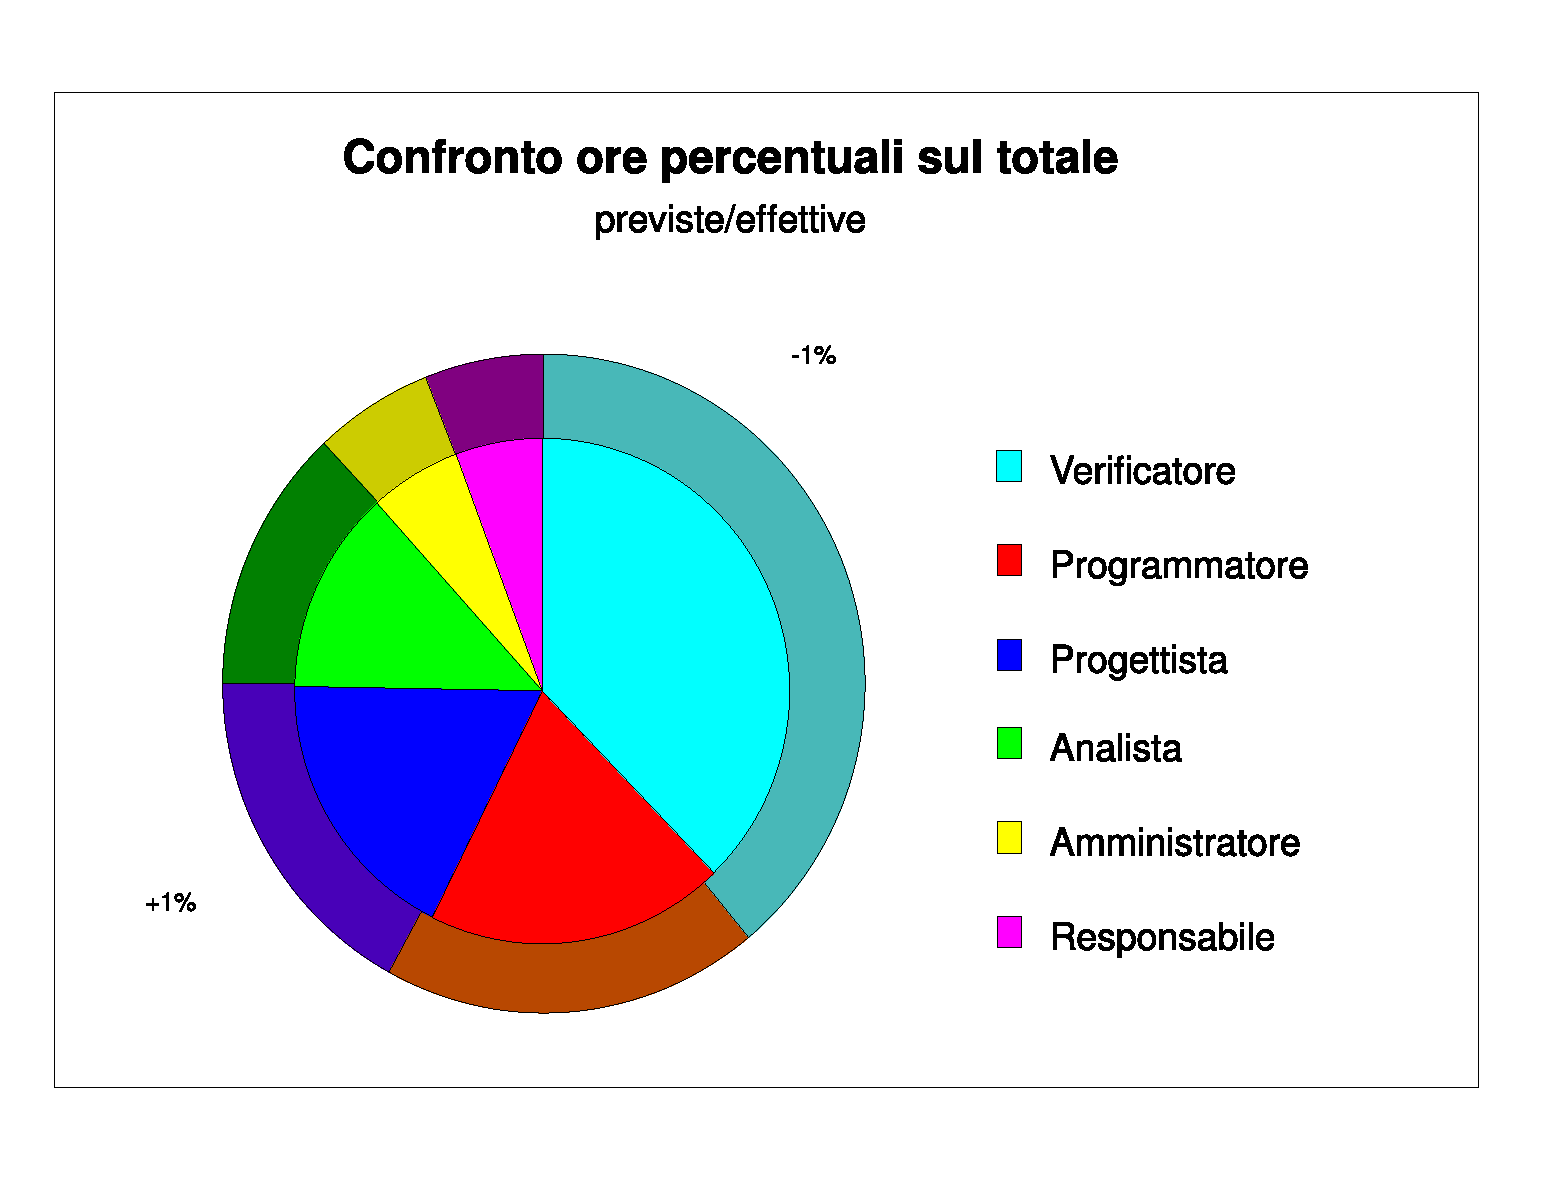
\includegraphics [width=1\textwidth] {progetto/oreperc.eps}
\end{center}


\section{Assegnazione dei ruoli e delle ore a ciascun membro}
Nelle seguenti tabelle vediamo la ripartizione delle ore nelle quattro macro-fasi rispetto ai ruoli di progetto. Per le fasi gi\`a concluse (analisi, progettazione e sviluppo) riportiamo le ore effettive indicando tra parentesi in che misura si discostano dalle previsioni iniziali.
\begin{table}[hbtp]
\large{
\begin{tabular}{l}
\Large{\textbf{\textsf{Fase di Analisi (Consuntivo) - 1}}} \\
\begin{tabular}{||p{3.5cm}||p{2cm}||p{2cm}||p{2cm}||p{2cm}||}
\hline
\textbf{Membro} & \textbf{Respon.} & \textbf{Ammin.} & \textbf{Analista}

& \textbf{Progett.}\\
\hline
{Appon Luca}&0&5&8 \footnotesize{(-1)}&3 \footnotesize{(+3)} \\ 
\hline 
{Bortolato Michele} &2&0&9&7 \footnotesize{(+5)}\\ 
\hline
{Carraro Filippo}&0&5&8&4 \footnotesize{(+4)} \\
\hline
{Meroi Mattia}&6&0&6 \footnotesize{(-1)}&3\footnotesize{(+3)}\\
\hline
{Tessarotto Marco} &0&0&9&7 \footnotesize{(+4)}\\
\hline
{Trivellato Alessia} &0&0&9&3 \footnotesize{(+3)} \\
\hline
{Trivellato Elena} &2&0&9&2 \footnotesize{(+2)} \\
\hline
{Totale}& 10&10&58 \footnotesize{(-2)}&29 \footnotesize{(+24)} \\
\hline

\end{tabular} \\
\end{tabular}
}
\end{table}

\begin{table}[hbtp]
\large{
\begin{tabular}{l}
\Large{\textbf{\textsf{Fase di analisi (Consuntivo) - 2}}} \\
\begin{tabular}{||p{3.5cm}||p{2cm}||p{2cm}||p{2cm}||p{2cm}||}
\hline
\textbf{Membro} & \textbf{Program} & \textbf{Verif.} & \textbf{Totale}\\ \hline
{Appon Luca}&0&3&17 \\ \hline 
{Bortolato Michele} &0&3&16\\ \hline
{Carraro Filippo}&0&3&16 \\ \hline
{Meroi Mattia}&0&4&17\\ \hline
{Tessarotto Marco} &0&4&16\\ \hline
{Trivellato Alessia} &0&7&16 \\ \hline
{Trivellato Elena} &0&6&17 \\ \hline
{Totale} &0&30&115 \\ \hline
\end{tabular} \\
\end{tabular}
}
\end{table}


\begin{table}[hbtp]
\large{
\begin{tabular}{l}
\Large{\textbf{\textsf{Fase di Progettazione (Consuntivo) - 1}}} \\
\begin{tabular}{||p{3.5cm}||p{2cm}||p{2cm}||p{2cm}||p{2cm}||}
\hline

\textbf{Membro} & \textbf{Respon.} & \textbf{Ammin.} & \textbf{Analista}
& \textbf{Progett.}\\
\hline
{Appon Luca}&4&0&2&8 \footnotesize{(-2)} \\ 
\hline 
{Bortolato Michele} &4&0&2&8 \footnotesize{(-2)}\\ 
\hline
{Carraro Filippo}&0&0&4&9 \footnotesize{(-3)} \\
\hline
{Meroi Mattia}&0&5&3&8 \footnotesize{(-2)}\\
\hline
{Tessarotto Marco} &0&0&4&9 \footnotesize{(-1)}\\
\hline
{Trivellato Alessia} &0&5&2&9 \footnotesize{(-3)} \\
\hline
{Trivellato Elena} &2&0&3&9 \footnotesize{(-2)} \\
\hline
{Totale}& 10&10&20&60 \footnotesize{(-15)} \\
\hline

\end{tabular} \\
\end{tabular}
}
\end{table}

\begin{table}[hbtp]
\large{
\begin{tabular}{l}
\Large{\textbf{\textsf{Fase di Progettazione (Consuntivo) - 2}}} \\
\begin{tabular}{||p{3.5cm}||p{2cm}||p{2cm}||p{2cm}||p{2cm}||}
\hline

\textbf{Membro} & \textbf{Program} & \textbf{Verif.} & \textbf{Totale}\\
\hline
{Appon Luca}&0&5&21 \\ 
\hline 
{Bortolato Michele} &2 \footnotesize{(+2)}&6&22\\ 
\hline
{Carraro Filippo}&2 \footnotesize{(+2)}&5&21 \\
\hline
{Meroi Mattia}&0&3&21\\
\hline
{Tessarotto Marco} &4 \footnotesize{(-1)}&3&22\\
\hline
{Trivellato Alessia} &1 \footnotesize{(+1)}&3&22 \\
\hline
{Trivellato Elena} &1 \footnotesize{(+1)}&5&21 \\
\hline
{Totale}&10 \footnotesize{(+5)}&30&150 \\
\hline

\end{tabular} \\
\end{tabular}
}
\end{table}


\begin{table}[hbtp]
\large{
\begin{tabular}{l}
\Large{\textbf{\textsf{Fase di Sviluppo (Consuntivo) - 1}}} \\
\begin{tabular}{||p{3.5cm}||p{2cm}||p{2cm}||p{2cm}||p{2cm}||}
\hline
\textbf{Membro} & \textbf{Respon.} & \textbf{Ammin.} & \textbf{Analista} & \textbf{Progett.}\\ \hline
{Appon Luca}&0&0&2&5 \\ \hline 
{Bortolato Michele} &0&2&0&3\\ \hline
{Carraro Filippo}&3\footnotesize{(-2)}&0&0&6\footnotesize{(+2)} \\ \hline
{Meroi Mattia}&0&0&3&3\footnotesize{(-1)}\\ \hline
{Tessarotto Marco} &2\footnotesize{(-3)}&2\footnotesize{(-4)}&0&2\footnotesize{(-1)}\\ \hline
{Trivellato Alessia} &2\footnotesize{(+2)}&4\footnotesize{(+2)}&0&3 \\ \hline
{Trivellato Elena} &0&0&0&3 \\ \hline
{Totale}& 7\footnotesize{(-3)}&8\footnotesize{(-2)}&5&25 \\ \hline
\end{tabular} \\
\end{tabular}
}
\end{table}
\begin{table}[hbtp]
\large{
\begin{tabular}{l}
\Large{\textbf{\textsf{Fase di Sviluppo (Consuntivo) - 2}}} \\
\begin{tabular}{||p{3.5cm}||p{2cm}||p{2cm}||p{2cm}||p{2cm}||}
\hline
\textbf{Membro} & \textbf{Program} & \textbf{Verif.} & \textbf{Totale}\\ \hline
{Appon Luca}&10&9\footnotesize{(-3)}&26\footnotesize{(-3)} \\ \hline 
{Bortolato Michele} &12&11\footnotesize{(+1)}&28\footnotesize{(+1)}\\ \hline
{Carraro Filippo}&8&10\footnotesize{(-2)}&27\footnotesize{(-2)} \\ \hline
{Meroi Mattia}&12&8\footnotesize{(-1)}&26\footnotesize{(-2)}\\ \hline
{Tessarotto Marco} &4&18\footnotesize{(+7)}&28\footnotesize{(-1)}\\ \hline
{Trivellato Alessia} &7&11\footnotesize{(-6)}&26\footnotesize{(-3)} \\ \hline
{Trivellato Elena} &6\footnotesize{(-1)}&18\footnotesize{(-1)}&27\footnotesize{(-2)} \\ \hline
{Totale}& 59\footnotesize{(-1)}&85\footnotesize{(-5)}&189\footnotesize{(-11)} \\ \hline
\end{tabular} \\
\end{tabular}
}
\end{table}


\begin{table}[hbtp]
\large{
\begin{tabular}{l}
\Large{\textbf{\textsf{Fase di Verifica (Preventivo) - 1}}} \\
\begin{tabular}{||p{3.5cm}||p{2cm}||p{2cm}||p{2cm}||p{2cm}||} \hline
\textbf{Membro} & \textbf{Respon.} & \textbf{Ammin.} & \textbf{Analista} & \textbf{Progett.}\\ \hline
{Appon Luca}&2&0&0&0 \\ \hline 
{Bortolato Michele} &0&5&0&0\\ \hline
{Carraro Filippo}&0&0&0&0 \\ \hline
{Meroi Mattia}&0&0&0&0\\ \hline
{Tessarotto Marco} &0&0&0&0\\ \hline
{Trivellato Alessia} &5&0&0&0 \\ \hline
{Trivellato Elena} &2&5&0&0 \\ \hline
{Totale}& 9&10&0&0 \\ \hline
\end{tabular} \\
\end{tabular}
}
\end{table}

\begin{table}[hbtp]
\large{
\begin{tabular}{l}
\Large{\textbf{\textsf{Fase di Verifica (Preventivo) - 2}}} \\
\begin{tabular}{||p{3.5cm}||p{2cm}||p{2cm}||p{2cm}||p{2cm}||} \hline
\textbf{Membro} & \textbf{Program} & \textbf{Verif.} & \textbf{Totale}\\ \hline
{Appon Luca}&6&16&24 \\ \hline
{Bortolato Michele} &3&17&25\\ \hline
{Carraro Filippo}&10&14&24 \\ \hline
{Meroi Mattia}&7&17&24\\ \hline
{Tessarotto Marco} &7&17&249\\ \hline
{Trivellato Alessia} &11&8&24 \\ \hline
{Trivellato Elena} &11&6&24 \\ \hline
{Totale} &55&95&169 \\ \hline
\end{tabular} \\
\end{tabular}
}
\end{table}

\newpage

\section{Carico totale di ore per ciascun componente}
In questa sezione vediamo in che misura (numero di ore) ogni componente collabora alla 
realizzazione del progetto in ogni macrofase e globalmente. Come prima, a fianco delle ore effettive indicheremo lo scostamento dalle previsioni.
Il bilancio delle ore ``previste-effettive'' aveva evidenziato un leggero aumento del carico complessivo di lavoro per ciascun membro del gruppo al termine della fase precedente. In fase di sviluppo invece assistiamo alla forzata riduzione del numero globale delle ore, al fine rientrare nei costi pattuiti con il committente. Tale riduzione non \`e stata distribuita in maniera omogenea tra i componenti del gruppo, pertanto alcuni hanno beneficiato pi\`u di altri della diminuzione del carico di lavoro. La Happycode si impegna, per quanto possibile, a tenere conto di ci\`o nella fase di verifica, richiedendo maggior impegno a coloro che hanno dedicato alla fase di sviluppo un numero minore di ore e alleggerendo invece il carico di lavoro di coloro che hanno fin qui contribuito di pi\`u allo sviluppo del software.


\begin{table}[hbtp]
\large{
\begin{tabular}{l}
\Large{\textbf{\textsf{Carico totale delle risorse (Consuntivo al 15/02/08) - 1}}} \\

\begin{tabular}{||p{3.5cm}||p{2cm}||p{2cm}||p{2cm}||p{2cm}||}
\hline
\textbf{Membro} & \textbf{Respon.} & \textbf{Ammin.} & \textbf{Analista}
& \textbf{Progett.}\\
\hline
{Appon Luca}&6&5&12 \footnotesize{(-1)}&16 \footnotesize{(+1)} \\ 
\hline 
{Bortolato Michele} &6&7&11&18 \footnotesize{(+3)}\\ 
\hline
{Carraro Filippo}&3\footnotesize{(-2)}&5&12&19 \footnotesize{(+3)} \\
\hline
{Meroi Mattia}&6&5&12 \footnotesize{(-1)}&14\\
\hline
{Tessarotto Marco} &2\footnotesize{(-3)}&2\footnotesize{(-4)}&13&18 \footnotesize{(+2)}\\
\hline
{Trivellato Alessia} &7\footnotesize{(+2)}&9\footnotesize{(+2)}&11&15\footnotesize{(-3)} \\
\hline
{Trivellato Elena} &6&5&12&14\footnotesize{(-2)} \\
\hline
{Totale}& 36\footnotesize{(-3)}&38\footnotesize{(-2)}&83\footnotesize{(-2)}&114 \footnotesize{(+9)} \\
\hline



\end{tabular} \\
\end{tabular}
}
\end{table}

\begin{table}[hbtp]
\large{
\begin{tabular}{l}
\Large{\textbf{\textsf{Carico totale delle risorse (Consuntivo al 15/02/08) - 2}}} \\

\begin{tabular}{||p{3.5cm}||p{2cm}||p{2cm}||p{2cm}||p{2cm}||}
\hline
\textbf{Membro} & \textbf{Program} & \textbf{Verif.} & \textbf{Totale}\\
\hline
{Appon Luca}&16&33\footnotesize{(-3)}&88\footnotesize{(-3)} \\ 
\hline 
{Bortolato Michele} &17 \footnotesize{(+2)}&37\footnotesize{(+1)}&96 \footnotesize{(+6)}\\ 
\hline
{Carraro Filippo}&20 \footnotesize{(+2)}&32\footnotesize{(-2)}&91\footnotesize{(-23)} \\
\hline
{Meroi Mattia}&19&32\footnotesize{(-1)}&88\footnotesize{(-2)}\\
\hline
{Tessarotto Marco} &15 \footnotesize{(-1)}&42\footnotesize{(+7)}&92 \footnotesize{(+1)}\\
\hline
{Trivellato Alessia} &19 \footnotesize{(+1)}&29\footnotesize{(-6)}&90 \footnotesize{(-1)} \\
\hline
{Trivellato Elena} &18&35\footnotesize{(-1)}&90 \footnotesize{(-1)} \\
\hline
{Totale} &124 \footnotesize{(+4)}&240\footnotesize{(-5)}&636 \footnotesize{(+2)} \\
\hline

\end{tabular} \\
\end{tabular}
}
\end{table}


\chapter{Costi}
\section{Costo orario per ogni ruolo}
Evidenziamo il costo orario di ciascun ruolo di progetto
\begin{table}[hbtp]
\large{
\begin{tabular}{l}
\Large{\textbf{\textsf{Tabella dei costi orari}}} \\

\begin{tabular}{||p{6cm}||p{5cm}||}
\hline
\textbf{Ruoli} & \textbf{Costo orario in Euro}\\
\hline
{Responsabile}&30,00\\ 
\hline 
{Amministratore} &18,00\\ 
\hline
{Analista} &25,00 \\
\hline
{Progettista} &20,00 \\
\hline
{Programmatore} &15,00\\
\hline
{Verificatore} &15,00 \\
\hline

\end{tabular} \\
\end{tabular}
}
\end{table}

\section{Costo totale per ogni ruolo}
Evidenziamo il costo totale di ciascun ruolo di progetto e la sua incidenza percentuale sul totale di spesa prevista. Nella fase precedente il costo totale con i dati effettivi delle prime fasi superava di 205,00 euro la spesa prevista. A fase di sviluppo conclusa invece, il prezzo previsto per il prodotto finito, tenuto conto delle ore gi� dedicate a questo progetto, e di 11,00 euro inferiore alle previsioni iniziali. Le modifiche percentuali inferiori ad 1 sono visibili nel grafico successivo ma non vengono riportate in tabella.

\begin{table}[hbtp]
\large{

\begin{tabular}{l}
\Large{\textbf{\textsf{Tabella dei costi Totali (Consuntivo al 15/02/08)}}} \\
\begin{tabular}{||p{4cm}||p{4cm}||p{4cm}||}
\hline
\textbf{Ruoli} & \textbf{Costo Totale}& \textbf{Costo Percentuale}\\
\hline
{Responsabile}&1.080,00\footnotesize{(-90,00)}&9 \footnotesize{(-1)}\\ 
\hline 
{Amministratore} &684,00\footnotesize{(-36,00)}&6\\ 
\hline
{Analista} &2.075,00 \footnotesize{(-50,00)}&18\footnotesize{(+1)} \\
\hline
{Progettista} &2.280,00 \footnotesize{(+180,00)}&20 \footnotesize{(-2)} \\
\hline
{Programmatore} &1.860,00 \footnotesize{(+60,00)}&16 \footnotesize{(+1)}\\
\hline
{Verificatore} &3.600,00\footnotesize{(-75,00)}&31 \footnotesize{(+1)} \\
\hline
{Totale} &11.579,00 \footnotesize{(-11,00)}&100 \\
\hline

\end{tabular} \\
\end{tabular}
}
\end{table}

\newpage
Evidenziamo, attraverso un grafico, come il costo di ciascun ruolo incida in percentuale sul totale. Adottiamo ancora una volta la convenzione secondo la quale il cerchio pi\`u esterno con colori pi\`u scuri rappresenta i dati previsti, mentre i dati effettivi sono quelli interni di colore pi\`u chiaro:
\begin{center}
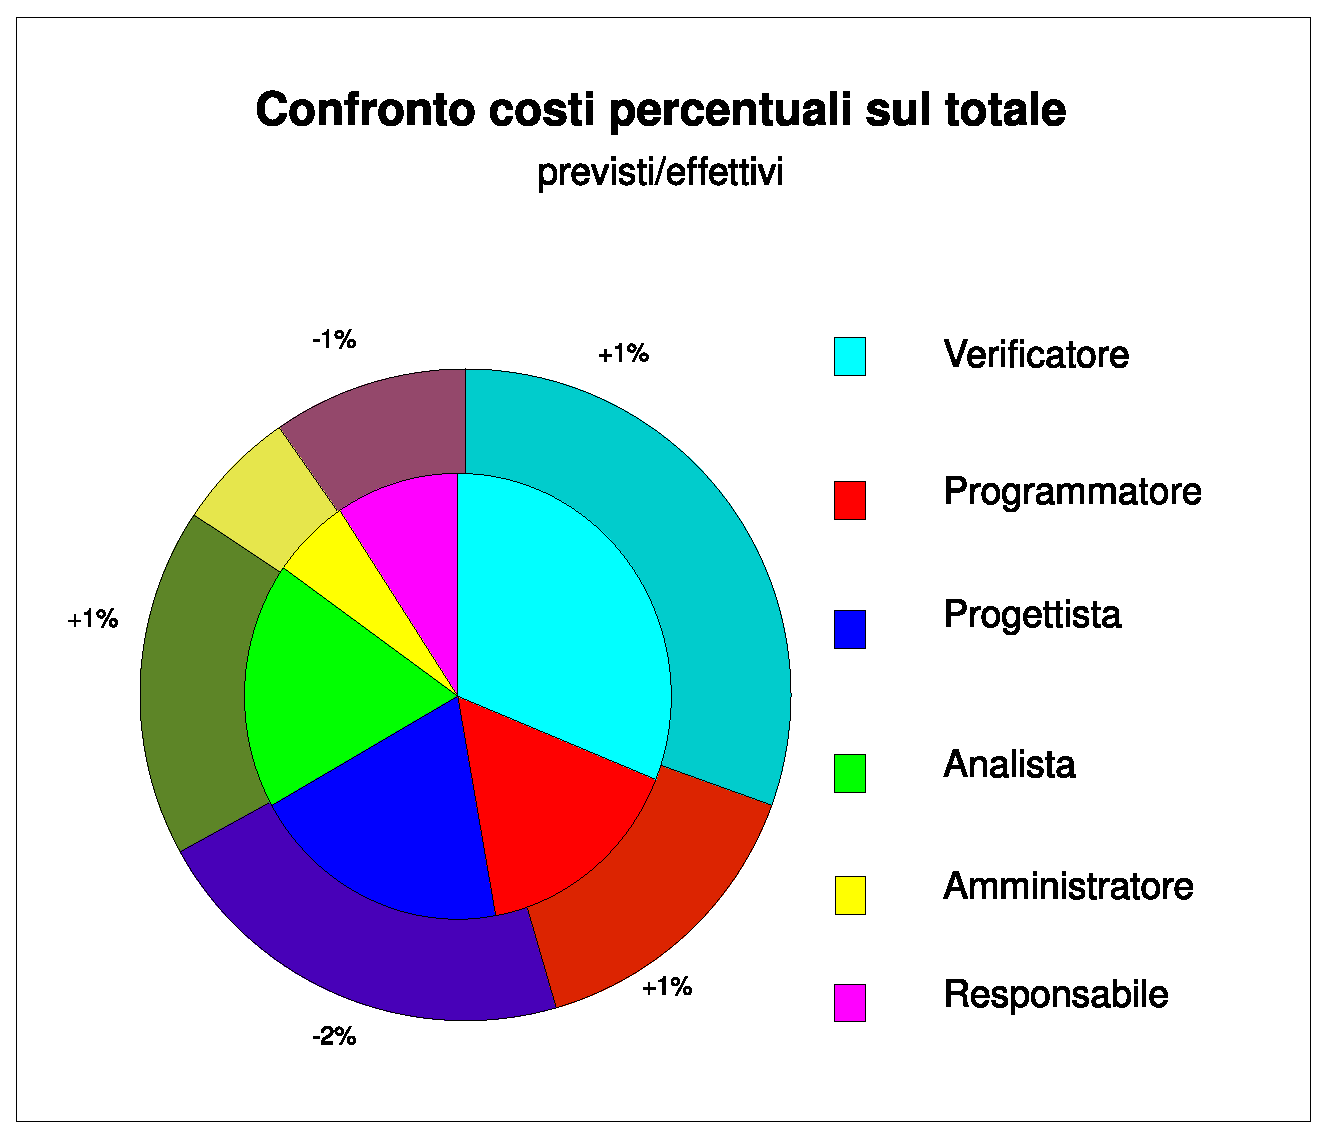
\includegraphics [width=1\textwidth] {progetto/costiperc.eps}
\end{center}


\chapter{Diagramma di Gantt}
Alleghiamo due files denominati rispettivamente:
\begin {itemize} 
\item Gantt\_RQ.png che rappresenta l'impiego delle risorse nel tempo visualizzate giorno per giorno;
\item Gantt\_sett\_RQ.png che invece mostra l'impiego delle risorse pi\`u globalmente organizzato per settimane.
\end{itemize}


\end{document}
